\documentclass[12pt, fullpage,letterpaper]{article}

\usepackage[margin=1in]{geometry}
\usepackage{url}
\usepackage{amsmath}
\usepackage{amssymb}
\usepackage{xspace}
\usepackage{graphicx}
\usepackage{hyperref}
\usepackage{listings}

\newcommand{\semester}{Spring 2019}
\newcommand{\assignmentId}{2}
\newcommand{\releaseDate}{11 Feb, 2019}
\newcommand{\dueDate}{11:59pm, 25 Feb, 2019}

\newcommand{\bx}{{\bf x}}
\newcommand{\bw}{{\bf w}}

\title{CS 5350/6350: Machine Learning \semester}
\author{Homework \assignmentId}
\date{Handed out: \releaseDate\\
	Due: \dueDate}


\title{CS 5350/6350: Machine Learning \semester}
\author{Homework \assignmentId}
\date{Handed out: \releaseDate\\
  Due date: \dueDate}

\begin{document}
\maketitle

% Math commands by Thomas Minka
\newcommand{\var}{{\rm var}}
\newcommand{\Tr}{^{\rm T}}
\newcommand{\vtrans}[2]{{#1}^{(#2)}}
\newcommand{\kron}{\otimes}
\newcommand{\schur}[2]{({#1} | {#2})}
\newcommand{\schurdet}[2]{\left| ({#1} | {#2}) \right|}
\newcommand{\had}{\circ}
\newcommand{\diag}{{\rm diag}}
\newcommand{\invdiag}{\diag^{-1}}
\newcommand{\rank}{{\rm rank}}
% careful: ``null'' is already a latex command
\newcommand{\nullsp}{{\rm null}}
\newcommand{\tr}{{\rm tr}}
\renewcommand{\vec}{{\rm vec}}
\newcommand{\vech}{{\rm vech}}
\renewcommand{\det}[1]{\left| #1 \right|}
\newcommand{\pdet}[1]{\left| #1 \right|_{+}}
\newcommand{\pinv}[1]{#1^{+}}
\newcommand{\erf}{{\rm erf}}
\newcommand{\hypergeom}[2]{{}_{#1}F_{#2}}

% boldface characters
\renewcommand{\a}{{\bf a}}
\renewcommand{\b}{{\bf b}}
\renewcommand{\c}{{\bf c}}
\renewcommand{\d}{{\rm d}}  % for derivatives
\newcommand{\e}{{\bf e}}
\newcommand{\f}{{\bf f}}
\newcommand{\g}{{\bf g}}
\newcommand{\h}{{\bf h}}
%\newcommand{\k}{{\bf k}}
% in Latex2e this must be renewcommand
\renewcommand{\k}{{\bf k}}
\newcommand{\m}{{\bf m}}
\newcommand{\mb}{{\bf m}}
\newcommand{\n}{{\bf n}}
\renewcommand{\o}{{\bf o}}
\newcommand{\p}{{\bf p}}
\newcommand{\q}{{\bf q}}
\renewcommand{\r}{{\bf r}}
\newcommand{\s}{{\bf s}}
\renewcommand{\t}{{\bf t}}
\renewcommand{\u}{{\bf u}}
\renewcommand{\v}{{\bf v}}
\newcommand{\w}{{\bf w}}
\newcommand{\x}{{\bf x}}
\newcommand{\y}{{\bf y}}
\newcommand{\z}{{\bf z}}
%s\newcommand{\l}{\boldsymbol{l}}
\newcommand{\A}{{\bf A}}
\newcommand{\B}{{\bf B}}
\newcommand{\C}{{\bf C}}
\newcommand{\D}{{\bf D}}
\newcommand{\E}{{\bf E}}
\newcommand{\F}{{\bf F}}
\newcommand{\G}{{\bf G}}
\renewcommand{\H}{{\bf H}}
\newcommand{\I}{{\bf I}}
\newcommand{\J}{{\bf J}}
\newcommand{\K}{{\bf K}}
\renewcommand{\L}{{\bf L}}
\newcommand{\M}{{\bf M}}
\newcommand{\N}{\mathcal{N}}  % for normal density
%\newcommand{\N}{{\bf N}}
\renewcommand{\O}{{\bf O}}
\renewcommand{\P}{{\bf P}}
\newcommand{\Q}{{\bf Q}}
\newcommand{\R}{{\bf R}}
\renewcommand{\S}{{\bf S}}
\newcommand{\T}{{\bf T}}
\newcommand{\U}{{\bf U}}
\newcommand{\V}{{\bf V}}
\newcommand{\W}{{\bf W}}
\newcommand{\X}{{\bf X}}
\newcommand{\Y}{{\bf Y}}
\newcommand{\Z}{{\bf Z}}

% this is for latex 2.09
% unfortunately, the result is slanted - use Latex2e instead
%\newcommand{\bfLambda}{\mbox{\boldmath$\Lambda$}}
% this is for Latex2e
\newcommand{\bfLambda}{\boldsymbol{\Lambda}}

% Yuan Qi's boldsymbol
\newcommand{\bsigma}{\boldsymbol{\sigma}}
\newcommand{\balpha}{\boldsymbol{\alpha}}
\newcommand{\bpsi}{\boldsymbol{\psi}}
\newcommand{\bphi}{\boldsymbol{\phi}}
\newcommand{\boldeta}{\boldsymbol{\eta}}
\newcommand{\Beta}{\boldsymbol{\eta}}
\newcommand{\btau}{\boldsymbol{\tau}}
\newcommand{\bvarphi}{\boldsymbol{\varphi}}
\newcommand{\bzeta}{\boldsymbol{\zeta}}

\newcommand{\blambda}{\boldsymbol{\lambda}}
\newcommand{\bLambda}{\mathbf{\Lambda}}
\newcommand{\bOmega}{\mathbf{\Omega}}
\newcommand{\bomega}{\mathbf{\omega}}
\newcommand{\bPi}{\mathbf{\Pi}}

\newcommand{\btheta}{\boldsymbol{\theta}}
\newcommand{\bpi}{\boldsymbol{\pi}}
\newcommand{\bxi}{\boldsymbol{\xi}}
\newcommand{\bSigma}{\boldsymbol{\Sigma}}

\newcommand{\bgamma}{\boldsymbol{\gamma}}
\newcommand{\bGamma}{\mathbf{\Gamma}}

\newcommand{\bmu}{\boldsymbol{\mu}}
\newcommand{\1}{{\bf 1}}
\newcommand{\0}{{\bf 0}}

% \newcommand{\comment}[1]{}

\newcommand{\bs}{\backslash}
\newcommand{\ben}{\begin{enumerate}}
\newcommand{\een}{\end{enumerate}}

 \newcommand{\notS}{{\backslash S}}
 \newcommand{\nots}{{\backslash s}}
 \newcommand{\noti}{{\backslash i}}
 \newcommand{\notj}{{\backslash j}}
 \newcommand{\nott}{\backslash t}
 \newcommand{\notone}{{\backslash 1}}
 \newcommand{\nottp}{\backslash t+1}
% \newcommand{\notz}{\backslash z}

\newcommand{\notk}{{^{\backslash k}}}
%\newcommand{\noti}{{^{\backslash i}}}
\newcommand{\notij}{{^{\backslash i,j}}}
\newcommand{\notg}{{^{\backslash g}}}
\newcommand{\wnoti}{{_{\w}^{\backslash i}}}
\newcommand{\wnotg}{{_{\w}^{\backslash g}}}
\newcommand{\vnotij}{{_{\v}^{\backslash i,j}}}
\newcommand{\vnotg}{{_{\v}^{\backslash g}}}
\newcommand{\half}{\frac{1}{2}}
\newcommand{\msgb}{m_{t \leftarrow t+1}}
\newcommand{\msgf}{m_{t \rightarrow t+1}}
\newcommand{\msgfp}{m_{t-1 \rightarrow t}}

\newcommand{\proj}[1]{{\rm proj}\negmedspace\left[#1\right]}
\newcommand{\argmin}{\operatornamewithlimits{argmin}}
\newcommand{\argmax}{\operatornamewithlimits{argmax}}

\newcommand{\dif}{\mathrm{d}}
\newcommand{\abs}[1]{\lvert#1\rvert}
\newcommand{\norm}[1]{\lVert#1\rVert}

%miscellaneous symbols
\newcommand{\ie}{{{i.e.,}}\xspace}
\newcommand{\eg}{{{\em e.g.,}}\xspace}
\newcommand{\EE}{\mathbb{E}}
\newcommand{\VV}{\mathbb{V}}
\newcommand{\sbr}[1]{\left[#1\right]}
\newcommand{\rbr}[1]{\left(#1\right)}
\newcommand{\cmt}[1]{}


{\footnotesize
	\begin{itemize}
		\item You are welcome to talk to other members of the class about
		the homework. I am more concerned that you understand the
		underlying concepts. However, you should write down your own
		solution. Please keep the class collaboration policy in mind.
		
		\item Feel free to discuss the homework with the instructor or the TAs.
		
		\item Your written solutions should be brief and clear. You do not need to include original problem descriptions in your solutions. You need to
		show your work, not just the final answer, but you do \emph{not}
		need to write it in gory detail. Your assignment should be {\bf no
			more than 15 pages}. Every extra page will cost a point.
		
		\item Handwritten solutions will not be accepted.
		
		
		\item {\em Your code should run on the CADE machines}. You should
		include a shell script, {\tt run.sh}, that will execute your code
		in the CADE environment. Your code should produce similar output
		to what you include in your report.
		
		You are responsible for ensuring that the grader can execute the
		code using only the included script. If you are using an
		esoteric programming language, you should make sure that its
		runtime is available on CADE.
		
		\item Please do not hand in binary files! We will {\em not} grade
		binary submissions.
		
		\item The homework is due by \textbf{midnight of the due date}. Please submit
		the homework on Canvas.
		
	\end{itemize}
}


\section{Paper Problems [40 points + 6 bonus]}
\begin{enumerate}
\item~[5 points] We have derived the PAC guarantee for consistent learners (namely, the learners can produce a hypothesis that can 100\% accurately classify the training data). The PAC guarantee is described as follows. Let $H$ be the hypothesis space used by our algorithm. Let $C$ be the concept class we want to apply our learning algorithm to search for a target function in $C$. We have shown that,  with probability at least $1-\delta$, a hypothesis $h\in H$ that is consistent with a training set of $m$ examples will have the generalization error $\mathrm{err}_D(h) < \epsilon$ if 
\[
m > \frac{1}{\epsilon}\big(\log(|H|) + \log\frac{1}{\delta}\big).
\]

\begin{enumerate}
	\item~[2 points] Suppose we have two learning algorithms $L_1$ and $L_2$, which use hypothesis spaces $H_1$ and $H_2$ respectively. We know that $H_1$ is larger than $H_2$, \ie $|H_1| > |H_2|$.
	For each target function in $C$, we assume both algorithms can find a hypothesis consistent with the training data. 
	\begin{enumerate}
		\item~[1 point] According to Occam's Razor principle, which learning algorithm's  result hypothesis do you prefer? Why?
		\bigskip\newline
		Occam's Razor dictates that one always prefer the most simple model of something possible. Therefore I would prefer $H_1$, as it uses fewer attributes to describe something.
		\bigskip
		\item~[1 point]  How is this principle reflected in our PAC guarantee? Please use the above inequality to explain why we will prefer the corresponding result hypothesis. 
		\bigskip\newline
		Because $H_1$ is a smaller hypothesis space, a consistent learner will require fewer examples to achieve a certain amount of generalization error in comparison to the larger $H_2$, as defined by the PAC guarantee.
		\bigskip
	\end{enumerate}
	\item~[3 points] Let us investigate algorithm $L_1$. Suppose we have $n$ input features, and the size of the hypothesis space used by $L_1$ is $3^n$. Given $n=10$ features, if we want to guarantee a 95\% chance of learning a hypothesis of at least 90\% generalization accuracy, how many training examples at least do we need for $L_1$?
	\smallskip\newline
	$m > \frac{1}{\epsilon}\big(\log(|H|) + \log\frac{1}{\delta}\big)$
	
	$\frac{1}{0.9}\big(\log_2(3^{10}) + \log_2\frac{1}{(1-0.95)}\big) \approx 22.413 < m$
	
	At least 23 training examples are needed for $L_1$.
	\bigskip
\end{enumerate}

\item~[7 points] Let us check the PAC learnability for several concept classes. We assume that our learning algorithm can always result in a hypothesis consistent with the training data. We assume the hypothesis space $H$ is the same as the concept class $C$. Please determine whether the following concept classes are PAC learnable or not and prove your conclusions [Hint: please carefully check the definition of PAC learnability]. 
\begin{enumerate}
	\item~[1 points] Simple disjunctions out of $n$ binary variables
	\bigskip\newline
	This hypothesis space has size at most $2^n$. This being a finite number, some m can be chosen for any n such that the PAC learnability inequality is true.
	\bigskip
	\item~[1 points] $m$-of-$n$ rules (Note that $m$ is a fixed constant).  
	\item~[1 points] General conjunctions out of $n$ binary variables (``General'' means that negations are allowed to operator on each variable before the conjunction).
	\item~[2 points] General Boolean functions of $n$ binary variables. 
	\item~[2 points] Can ID3 algorithm \textit{efficiently} PAC learn the above concept classes? 
\end{enumerate}

\item~[5 points] In our lecture about AdaBoost algorithm, we introduced the definition of weighted error in each round $t$, 
\[
\epsilon_t = \frac{1}{2} - \frac{1}{2}\big(\sum_{i=1}^m D_t(i) y_i h_t(x_i)\big)
\]
where $D_t(i)$ is the weight of $i$-th training example, and $h_t(x_i)$ is the prediction of the weak classifier learned round $t$. Note that both $y_i$ and $h_t(x_i)$ belong to $\{1, -1\}$. Prove that equivalently,
\[
\epsilon_t = \sum_{y_i \neq h_t(x_i)} D_t(i).
\]

\bigskip
$\frac{1}{2} - \frac{1}{2}\big(\sum D_t(i) y_i h_t(x_i)\big)$

$\frac{1}{2}\big(1 - \sum D_t(i) y_i h_t(x_i)\big)$

$\frac{1}{2}\big(1 - \sum_{y_i = h_t(x_i)} D_t(i) + \sum_{y_i \neq h_t(x_i)} D_t(i)\big)$

$\frac{1}{2}\big(1 - \sum_{y_i = h_t(x_i)} D_t(i) + \sum_{y_i \neq h_t(x_i)} D_t(i) + (\sum_{y_i = h_t(x_i)} D_t(i) + \sum_{y_i \neq h_t(x_i)} D_t(i) - 1)\big)$

$\frac{1}{2}\big(1 - 1 + \sum_{y_i = h_t(x_i)}D_t(i) - \sum_{y_i = h_t(x_i)}D_t(i) + \sum_{y_i \neq h_t(x_i)}D_t(i) + \sum_{y_i \neq h_t(x_i)}D_t(i)\big)$

$\frac{1}{2}\big(2\sum_{y_i \neq h_t(x_i)}D_t(i)\big)$

$\epsilon_t = \sum_{y_i \neq h_t(x_i)} D_t(i).$

\bigskip

	\item~[8 points] Can you figure out an equivalent linear classifier and a decision tree for the following Boolean functions? For linear classifiers, please point out what the weight vector, the bias parameter and the hyperplane are. Note that the hyperplane is determined by an equality. If you cannot find out such a  linear classifier, please explain why. 
	\begin{enumerate}
		\item~[1 point] $f(x_1, x_2, x_3) = x_1 \lor x_2 \lor x_3$
		
		\bigskip
		$y = 1$ if $x_1 + x_2 + x_3 \ge 1$
		
		w = [1, 1, 1]
		
		b = -1
		
		plane: $-1 + x_1 + x_2 + x_3 = 0$
		
		Decision Tree:
		
		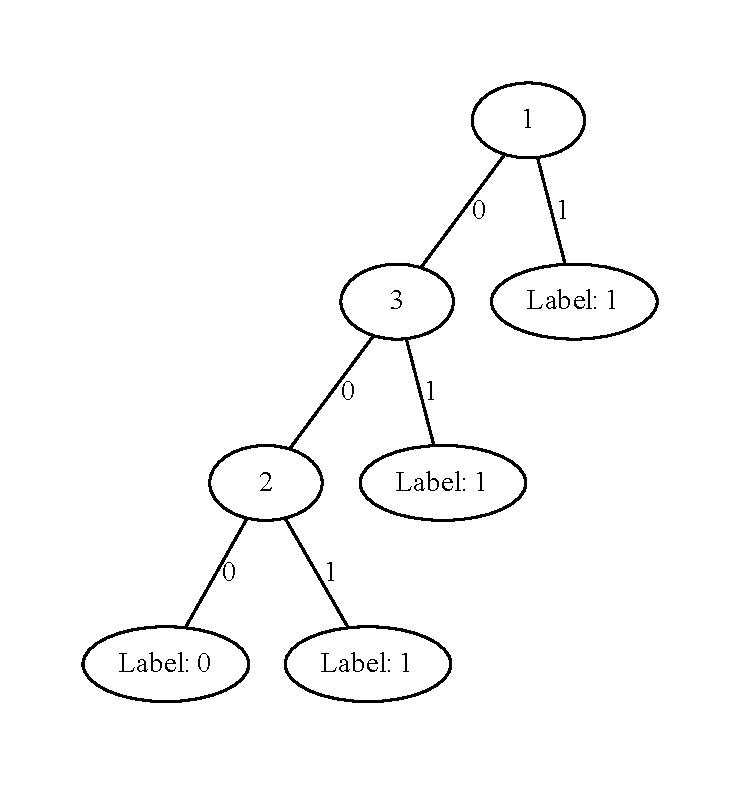
\includegraphics[scale=.5]{4a_tree.pdf}
		\bigskip\bigskip
		\item~[1 point] $f(x_1, x_2, x_3) = x_1 \land \neg x_2 \land \neg x_3$
		
		\bigskip
		$y = 1$ if $x_1 - x_2 - x_3 \ge 1$
		
		w = [1, -1, -1]
		
		b = -1
		
		plane: $-1 + x_1 - x_2 - x_3 = 0$
		
		Decision Tree:
		
		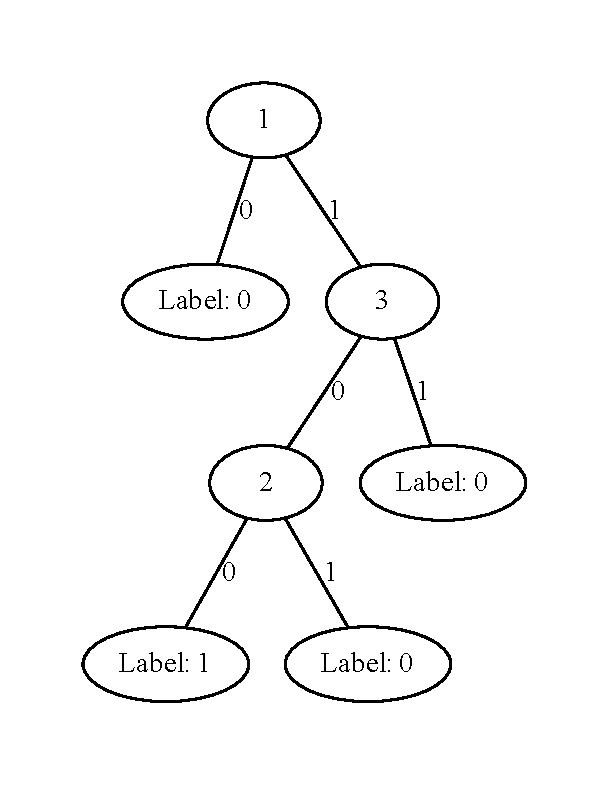
\includegraphics[scale=.5]{4b_tree.pdf}
		\bigskip
		\item~[1 point] $f(x_1, x_2, x_3) = \neg x_1 \lor \neg x_2 \lor \neg x_3$
		
		\bigskip
		$y = 1$ if $-x_1 - x_2 - x_3 \ge -2$
		
		w = [-1, -1, -1]
		
		b = 2
		
		plane: $2 - x_1 - x_2 - x_3 = 0$
		
		Decision Tree:
		
		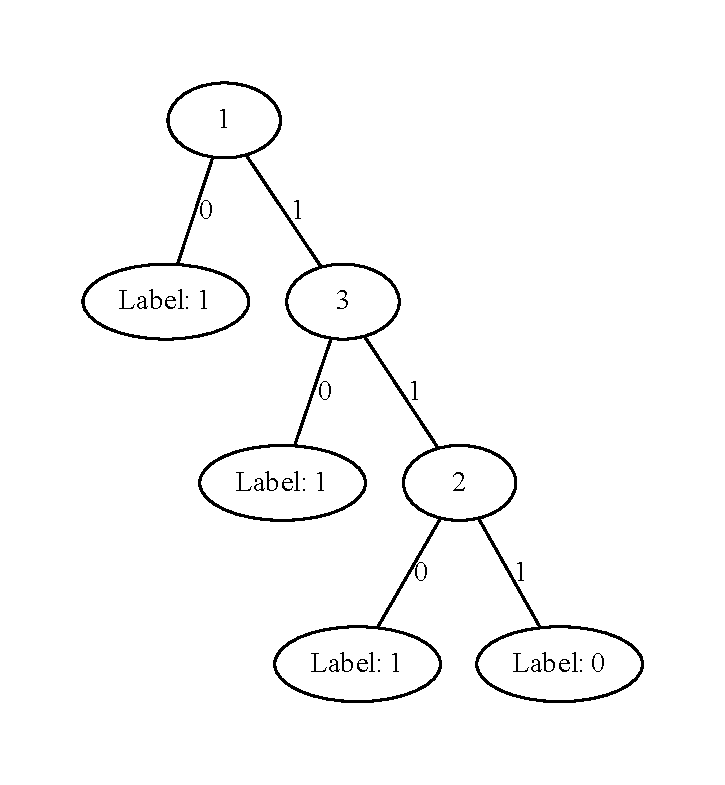
\includegraphics[scale=.5]{4c_tree.pdf}
		\bigskip 
		\item~[2 points] $f(x_1, x_2, x_3, x_4) = (x_1 \lor x_2) \land (x_3 \lor x_4)$
		
		\bigskip
		This boolean function is not linearly separable. At least two of the variables need to be true, however there is no way to specify which combinations of just two variables will create a true statement with a linear classifier.
		
		Decision Tree:
		
		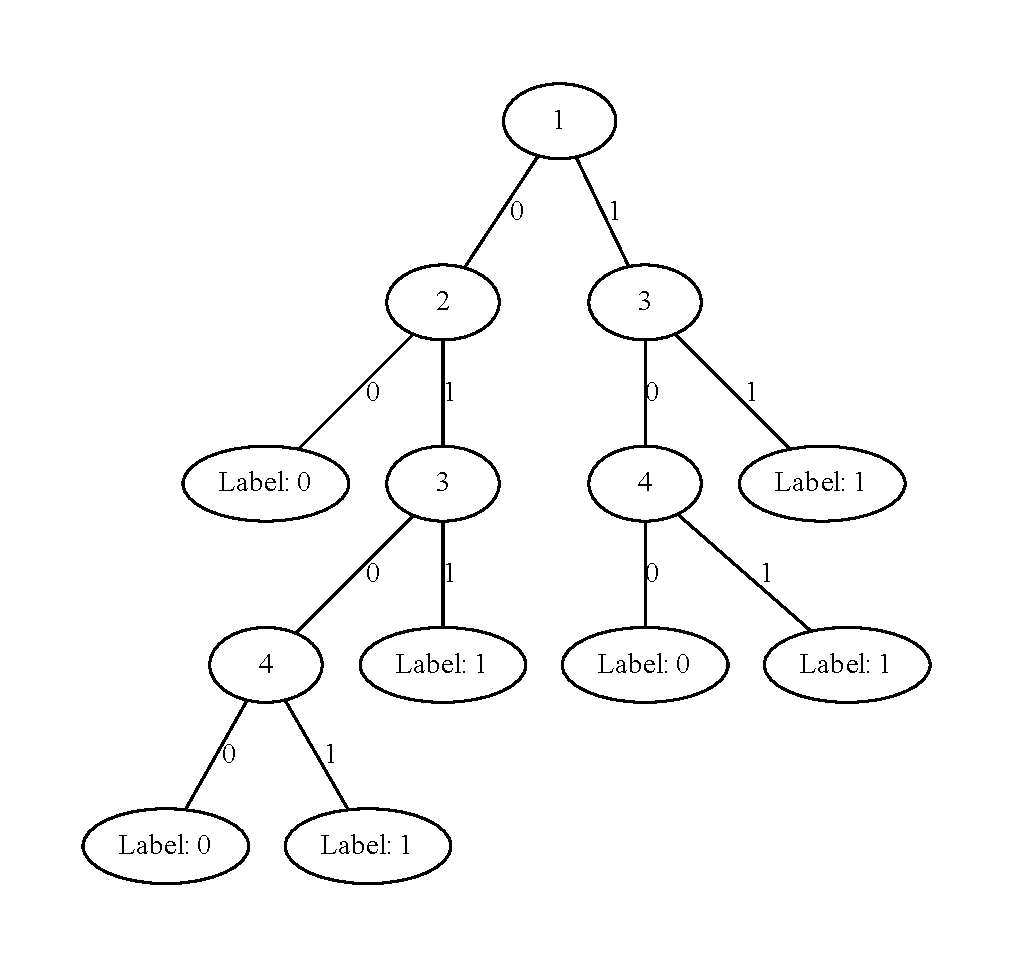
\includegraphics[scale=.4]{4d_tree.pdf}

		\item~[2 points] $f(x_1, x_2, x_3, x_4) = (x_1 \land x_2) \lor (x_3 \land x_4)$
		
		\bigskip
		This boolean function is not linearly separable for the same general reason as the previous one. At least two of the variables need to be true, however there is no way to specify which combinations of just two variables will create a true statement with a linear classifier.
		
		Decision Tree:
		
		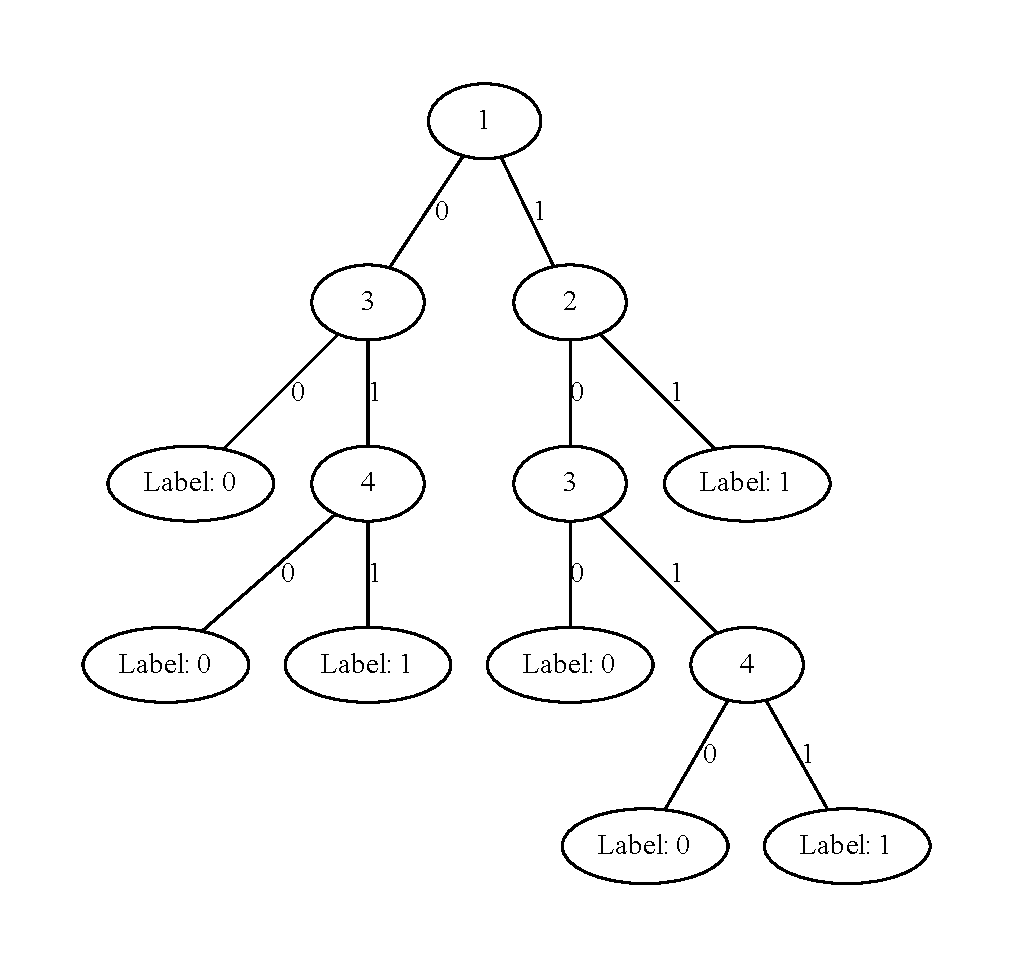
\includegraphics[scale=.4]{4e_tree.pdf}
		
		\item~[1 point] What do you conclude about the expressiveness of decision trees and linear classifiers? Why?
		\bigskip
		
		Decision trees can be far more expressive than linear classifiers when it comes to data with categorical attributes. Decision trees can encode every possible combination of values if enough depth and examples are given.
		
	\end{enumerate}
		
	
	\item~[6 points] The following boolean functions cannot be represented by linear classifiers. Can you work out some feature mapping such that, after mapping all the inputs of these functions into a higher dimensional space, you can easily identify a hyperplane that separates the inputs with different corresponding boolean function values? Please write down the separating hyperplane as well. 
	\begin{enumerate}
		\item $f(x_1, x_2) = (x_1 \land \neg x_2) \lor (\neg x_1 \land x_2)$
		
		Here I would add the third dimension $x_3$ such that $x_3 = x_1 \land x_2$. The resulting hyperplane would be $-1 + x_1 + x_2 + x_3 = 0$.
		
		\item $f(x_1, x_2) = (x_1 \land x_2) \lor (\neg x_1 \land \neg x_2)$
		
		Here I would add the third dimension $x_3$ such that $x_3 = (x_1 \land \neg x_2) \lor (\neg x_1 \land x_2)$. The resulting hyperplane would be $x_1 - x_2 - x_3 = 0$
		
		\item $f(x_1, x_2, x_3)$ is listed in the following table
		\begin{table}[h]
			\centering
			\begin{tabular}{ccc|c}
				$x_1$ & $x_2$ & $x_3$ &  $f(x_1, x_2, x_3)$\\ 
				\hline\hline
				0 & 0 & 0 & 0 \\ \hline
				0 & 0 & 1 & 1 \\ \hline
				0 & 1 & 0 & 1 \\ \hline
				1 & 0 & 0 & 1 \\ \hline
				0 & 1 & 1 & 0\\ \hline
				1 & 1 & 0 & 0\\ \hline
				1 & 0 & 1 & 0\\ \hline
				1 & 1 & 1 & 1\\ \hline
			\end{tabular}
		\end{table}
	
	Here I would add a 4th dimension $x_4$ such that $x_4 = (x_1 \land \neg x_2 \land \neg x_3) \lor (\neg x_1 \land x_2 \land \neg x_3) \lor (\neg x_1 \land \neg x_2 \land x_3) \lor (x_1 \land x_2 \land x_3)$. The resulting hyperplane would be $x_4 = 0.5$.
	
	\end{enumerate}
	
	\item~[\textbf{Bonus}]~[6 points]  Given two vectors $\x = [x_1,  x_2]$ and $\y=[y_1,  y_2]$, find a feature mapping $\phi(\cdot)$ for each of the following functions, such that the function is equal to the inner product between the mapped feature vectors, $\phi(\x)$ and $\phi(\y)$. For example, $(\x^\top \y)^0 = \phi(\x)^\top \phi(\y)$ where $\phi(\x) = [1]$ and $\phi(\y) = [1]$; $(\x^\top \y)^1 = \phi(\x)^\top \phi(\y)$ where $\phi(\x) = \x$ and $\phi(\y) = \y$. 
	\begin{enumerate}
		\item~[2 points] $(\x^\top \y)^2$
		
		$\phi(\x) = [x_1^2, 2x_1x_2, x_2^2]$
		
		$\phi(\y) = [y_1^2, y_1y_2, y_2^2]$
		\item~[2 points] $(\x^\top \y)^3$
		
		$\phi(\x) = [x_1^3, 3x_1^2x_2, 3x_1x_2^2, x_2^2]$
		
		$\phi(\y) = [y_1^3, y_1^2y_2, y_1y_2^2, y_2^3]$
		\item~[2 points] $(\x^\top \y)^k$ where $k$ is  any positive integer.
		
		Expand $(x_1y_1 + x_2y_2)^k$, then put the coefficients and $x$ terms into $\x$, and the $y$ terms into $\y$
	\end{enumerate}

\item~[9 points] Suppose we have the training data shown in Table \ref{tb:1}, from which we want to learn a linear regression model, parameterized by a weight vector $\w$ and a bias parameter $b$.  
\begin{table}[h]
	\centering
	\begin{tabular}{ccc|c}
		$x_1 $ & $x_2$ & $x_3$ &  $y$\\ 
		\hline\hline
		1 & -1 & 2 & 1 \\ \hline
		1 & 1 & 3 & 4 \\ \hline
		-1 & 1 & 0 & -1 \\ \hline
		1 & 2 & -4 & -2 \\ \hline
		3 & -1 & -1 & 0\\ \hline
	\end{tabular}
	\caption{Linear regression training data.}
	\label{tb:1}
\end{table}

\begin{enumerate}
	\item~[1 point] Write down the LMS (least mean square) cost function $J(\w, b)$. 
	
	$$J(\w, b) = \frac{1}{2} \sum_{i=1}^{m}(y_i - \w^T\x_i - b)^2$$
	\bigskip
	\item~[3 points] Calculate the gradient $\frac{\nabla J}{\nabla \w}$ and $\frac{\nabla J}{\nabla b}$
	
	$\frac{\nabla J}{\nabla \w} = [-\sum_{i=1}^{m}(y_i - \w^Tx_i - b)x_{i1}, \ldots, -\sum_{i=1}^{m}(y_i - \w^Tx_i - b)x_{id}]$
	
	$\frac{\nabla J}{\nabla b} = -\sum_{i=1}^{m}(y_i - \w^Tx_i - b)$	
	
	\begin{enumerate}
		\item when $\w = [0,0,0]^\top$ and $b = 0$;
		
		$\frac{\nabla J}{\nabla \w} = [-4, 2, -22]$
		
		$\frac{\nabla J}{\nabla b} = -2$
		\item when $\w = [-1,1,-1]^\top$ and $b = -1$;
		
		$\frac{\nabla J}{\nabla \w} = [-22, 16, -56]$
		
		$\frac{\nabla J}{\nabla b} = -10$
		\item when $\w = [1/2,-1/2,1/2]^\top$ and $b = 1$.
		
		$\frac{\nabla J}{\nabla \w} = [7.5, -4, -5]$
		
		$\frac{\nabla J}{\nabla b} = 4.5$
	\end{enumerate}
	\item~[2 points] What are the optimal $\w$ and $\b$ that minimize the cost function? 
	
	$\w = [1, 1, 1]^\top$
	
	$b = -1$
	
	\item~[3 points] Now, we want to use stochastic gradient descent to minimize $J(\w, b)$. We initialize $\w = \0$ and $b = 0$. We set the learning rate $r = 0.1$ and sequentially go through the $5$ training examples. Please list the stochastic gradient in each step and the updated $\w$ and $b$.
	
	\begin{enumerate}
		\item After s = [1, -1, 2]
		
		$\frac{\nabla J}{\nabla \w} = [-1, 1, -2]$
		
		$\frac{\nabla J}{\nabla b} = -1$
		
		$\w = [0.1, -0.1, 0.2]$
		
		$b = 0.1$
		\item After s = [1, 1, 3]
		
		$\frac{\nabla J}{\nabla \w} = [-3.3, -3.3, -9.9]$
		
		$\frac{\nabla J}{\nabla b} = -3.3$
		
		$\w = [0.43, 0.23, 1.19]$
		
		$b = 0.43$
		\item After s = [-1, 1, 0]
		
		$\frac{\nabla J}{\nabla \w} = [-1.23, 1.23, 0.0]$
		
		$\frac{\nabla J}{\nabla b} = 1.23$
		
		$\w = [0.553, 0.107, 1.19]$
		
		$b = 0.307$
		\item After s = [1, 2, -4]
		
		$\frac{\nabla J}{\nabla \w} = [-1.686, -3.372, 6.744]$
		
		$\frac{\nabla J}{\nabla b} = -1.686$
		
		$\w = [0.7216, 0.4442, 0.5156]$
		
		$b = 0.4756$
		\item After s = [3, -1, -1]
		
		$\frac{\nabla J}{\nabla \w} = [5.0418, -1.6806, -1.6806]$
		
		$\frac{\nabla J}{\nabla b} = 1.6806$
		
		$\w = [0.21742, 0.61226, 0.68366]$
		
		$b = 0.30754$
	\end{enumerate}
	
\end{enumerate}
\end{enumerate}

\section{Practice [60 points + 10 bonus]}
\begin{enumerate}
	\item~[2 Points] Update your machine learning library. Please check in your implementation of decision trees in HW1 to your GitHub repository. Remember last time you created a folder ``Decision Tree". You can commit your code into that folder. Please also supplement README.md with concise descriptions about how to use your code to learn decision trees (how to call the command, set the parameters, etc). Please create two folders ``Ensemble Learning" and ``Linear Regression''  in the same level as the folder ``Decision Tree''.  


\item~[36 points] We will implement the boosting and bagging algorithms based on decision trees.  Let us test them on the bank marketing dataset in HW1 (bank.zip in Canvas). We use the same approach to convert the numerical features into binary ones. That is, we choose the media (NOT the average) of the attribute values (in the training set) as the threshold, and examine if the feature is bigger (or less) than the threshold.  For simplicity, we treat ``unknown'' as a particular attribute value, and hence we do not have any missing attributes for both training and test.
\begin{enumerate}
	\item~[8 points] Modify your decision tree learning algorithm to learn decision stumps ---  trees with only two levels. Specifically, compute the information gain to select the best feature to split the data. Then for each subset, create a leaf node. Note that your decision stumps must support weighted training examples. Based on your decision stump learning algorithm, implement AdaBoost algorithm. Vary the number of iterations T from $1$ to $1000$, and examine the training and test errors. You should report the results in two figures. The first figure shows how the training and test errors vary along with T. The second figure shows the training and test errors of all the decision stumps learned in each iteration. What can you observe and conclude? You have had the results for a fully expanded decision tree in HW1. Comparing them with AdaBoost, what can you observe and conclude?
	
	\begin{center}
		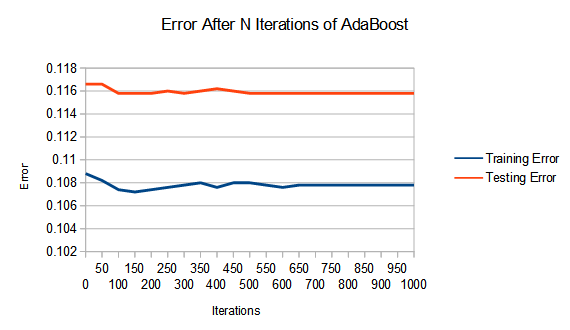
\includegraphics[scale=0.8]{adaboost_graph}
	\end{center}
	
	\begin{center}
		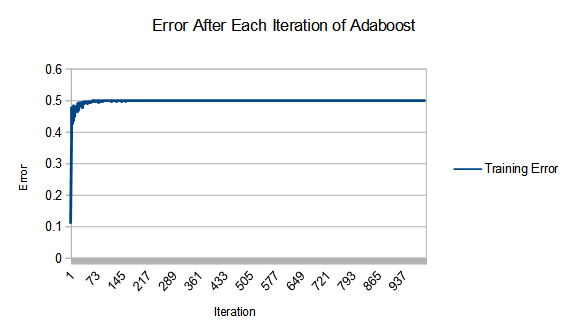
\includegraphics[scale=0.8]{adaboost_graph2}
	\end{center}
	
	The error of an individual stump quickly rises to near .5, but the overall error drops very slowly. A fully expanded tree is far more accurate on training data, but is prone to overfitting as AdaBoost had better testing error.
	
	\bigskip
	
	\item~[8 points] Based on your code of the decision tree learning algorithm (with information gain), implement a Bagged trees learning algorithm. Note that each tree should be fully expanded --- no early stopping or post pruning. Vary the number of trees from $1$ to $1000$, report how the training and test errors vary along with the tree number in a figure. Overall, are bagged trees better than a single tree? Are bagged trees better than Adaboost? 
	
	\begin{center}
		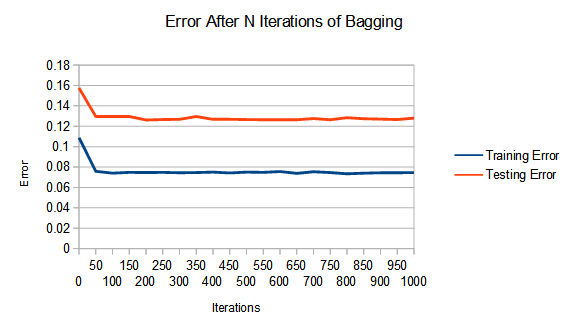
\includegraphics[scale=0.8]{bagging_graph}
	\end{center}
	
	Compared to a single tree, bagging is far less prone to overfitting. The training error is higher, but the testing error is lower. Bagged trees have a lower training error than AdaBoost, but a higher testing error, suggesting AdaBoost is even better at avoiding overfitting.
	
	\bigskip

	\item~[6 points] Through the bias and variance decomposition, we have justified why the bagging approach is more effective than a single classifier/predictor. Let us verify it in real data. Experiment with the following procedure.
	\begin{itemize}
		\item REPEAT for 100 times
		\item ~[STEP 1] Sample $1,000$ examples \textit{uniformly without replacement} from the training dataset
		\item ~[STEP 2] Run your bagged trees learning algorithm based on the $1,000$ training examples and learn $1000$ trees.
		\item END REPEAT 
		\item Now you have $100$ bagged predictors in hand. For comparison, pick the first tree in each run to get $100$ fully expanded trees (i.e. single trees). 
		\item 	For each of the test example, compute the predictions of the $100$ single trees. Take the average, subtract the ground-truth label, and take square to compute the bias term (see the lecture slides). Use all the predictions to compute the sample variance  as the approximation to the variance term (if you forget what the sample variance is, check it out 
		\href{http://www.randomservices.org/random/sample/Variance.html}{here}). You now obtain the bias and variance terms of a single tree learner for one test example. You will need to compute them for all the test examples and then take average as your final estimation of the bias and variance terms for the single decision tree learner. You can add the two terms to obtain the estimation of the general squared error (that is, expected error w.r.t test examples). Now use your $100$ bagged predictors to do the same thing and estimate the general bias and variance terms, as well as the general squared error.  Comparing the results of the single tree learner and the bagged trees, what can you conclude?  What causes the difference?  
	\end{itemize}
	\bigskip
	Single Tree bias: 0.37509816
	
	Single Tree variance: 0.36286184
	
	Single Tree general error: 0.73796
	
	\bigskip
	
	All Tree bias: 0.369140156808
	
	All Tree variance: 0.0582005373522
	
	All Tree general error: 0.4273406941602
	
	\bigskip
	
	The single tree and bagged trees have about the same bias, but the single trees have a much larger variance. This is because the bagged trees average the results of many decision trees.	
	
	\bigskip
	\item~[8 points] Implement the random forest algorithm as we discussed in our lecture. Vary the number of random trees from $1$ to $1000$. Note that you need to modify your tree learning algorithm to randomly select a subset of features before each split. Then use the information gain to select the best feature to split.  Vary the size of the feature subset from $\{2, 4, 6\}$. Note that if your feature subset happen to be all the features used before, simply resample the subset.  Report in a figure how the training and test errors vary along with the number of random trees for each feature subset size setting. How does the performance compare with bagged trees? 

	\begin{center}
		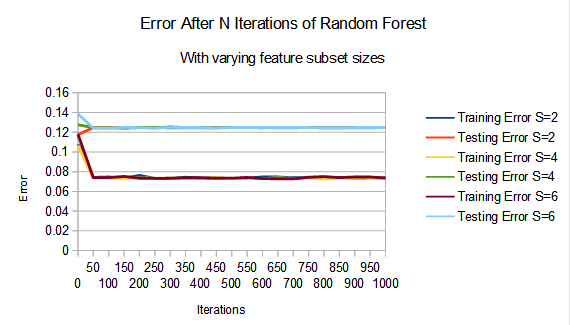
\includegraphics[scale=0.8]{forest_graph}
	\end{center}
	
	The training error is lower for the random forest than bagged trees, but the testing error is higher, so generally lower performance.
	
	\bigskip
	
	\item~[6 points] Following (c), estimate the bias and variance terms, and the squared error for a single random tree and the whole forest.  Comparing with the bagged trees, what do you observe? What can you conclude? 
\end{enumerate}

\item~[\textbf{Bonus}][10 points] In practice, to confirm the performance of your algorithm, you need to find multiple datasets for test (rather than one). You need to extract and process data by yourself. Now please use the credit default dataset in UCI repository \href{https://archive.ics.uci.edu/ml/datasets/default+of+credit+card+clients}{https://archive.ics.uci.edu/ml/datasets/default+of+credit+card+clients}. Randomly choose $24000$ examples for training and the remaining $6000$ for test. Feel free to deal with continuous features. Run bagged trees, random forest, and Adaboost with decision stumps algorithms for $1000$ iterations. Report in a figure how the training and test errors vary along with the number of iterations, as compared with a fully expanded single decision tree. Are the results consistent with the results you obtained from the bank dataset?

	\item~[22 points] We will implement the LMS method for a linear regression task. The dataset is from UCI repository (\url{https://archive.ics.uci.edu/ml/datasets/Concrete+Slump+Test}). The task is to predict the real-valued SLUMP of the concrete, with $7$ features. The features and output are listed in the file ``concrete/data-desc.txt''. The training data are stored in the file ``concrete/train.csv'', consisting of $53$ examples. The test data are stored in ``concrete/test.csv'', and comprise of $50$ examples. In both the training and testing datasets, feature values and outputs are separated by commas. 
	
	\begin{enumerate}
		\item~[8 points] Implement the batch gradient descent algorithm, and tune the learning rate $r$ to ensure the algorithm converges.  To examine convergence, you can watch the norm of the weight vector difference,  $\|w_{t} - w_{t-1}\|$,  at each step $t$.  if $\|w_{t} - w_{t-1}\|$ is  less than a tolerance level, say, $1e-6$, you can conclude that it converges. You can initialize your weight vector to be $\0$.  Please find an appropriate $r$ such that the algorithm converges. To tune $r$, you can start with a relatively big value, say, $r=1$, and then gradually decrease $r$, say $r=0.5, 0.25, 0.125, \ldots$, until you see the convergence. 
		Report the learned weight vector, and the learning rate $r$. Meanwhile, please record the cost function  value of the training data at each step, and then draw a figure shows how the cost function changes along with steps. Use your final weight vector to calculate  the cost function value of the test data. 
		
		\bigskip
		
		Final Weight Vector: [0.9211078533555084, 0.8078393812490983, 0.8734823089428027, 1.3139341774979179, 0.13385026003803402, 1.5984532026709113, 1.0198413438610812]
		
		Learning Rate: 0.0145
		
		Test Data Cost: 23.360684566927414
		
		\begin{center}
			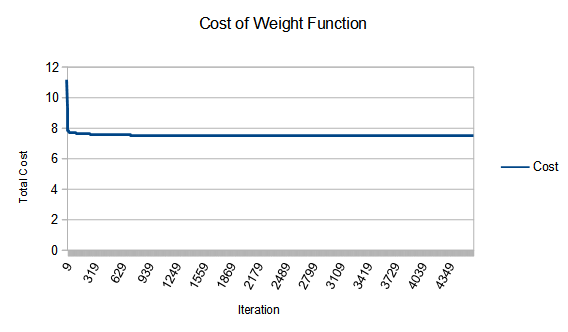
\includegraphics[scale=0.8]{batch_graph}
		\end{center}
		
		\item~[8 points] Implement the stochastic gradient descent (SGD) algorithm. You can initialize your weight vector to be $\0$. Each step, you randomly sample a training example, and then calculate the stochastic gradient to update the weight vector.  Tune the learning rate $r$ to ensure your SGD converges. To check convergence, you can calculate the cost function of the training data after each stochastic gradient update, and draw a figure showing how the cost function values vary along with the number of updates. At the beginning, your curve will oscillate a lot. However, with an appropriate $r$, as more and more updates are finished, you will see the cost function tends to converge. Please report the learned weight vector, and the learning rate you chose, and the cost function value of the test data with your learned weight vector.
				
		\bigskip
		
		Final Weight Vector: [0.5094767567479317, 0.025697021439722925, 0.5271134261486301, 0.8440867852320653, 0.19446188146527899, 0.58406310559173, 0.4617250233508782]
		
		Learning Rate: 0.1
		
		Test Data Cost: 20.444922087438073
		
		\begin{center}
			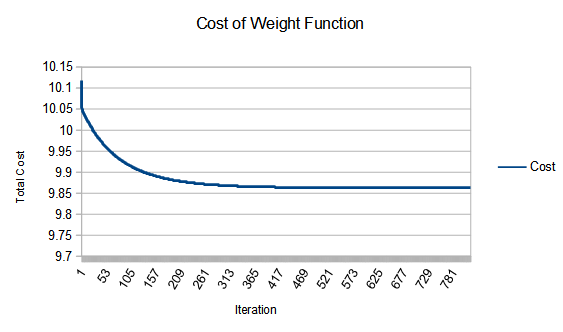
\includegraphics[scale=0.8]{stoch_graph}
		\end{center}
	
		\item~[6 points] We have discussed how to  calculate the optimal weight vector with an analytical form. Please calculate the optimal weight vector in this way. Comparing with the  weight vectors learned by batch gradient descent and stochastic gradient descent, what can you conclude? Why?
		
		\bigskip
		
		$\w* = [0.92154947, 0.80829428, 0.87397433, 1.3142877, 0.13392374, 1.59904727, 1.02029192]$
		
		The weight vector batch gradient descent converged on is very close to the optimal weight vector, while the stochastic version likely converged to a different local minimum. This is likely because the first few examples evaluated by the stochastic version moved the weight vector very close to the local minimum it ended on.
		
	\end{enumerate}

\end{enumerate}

\end{document}
%%% Local Variables:
%%% mode: latex
%%% TeX-master: t
%%% End:
